\documentclass{report}
\usepackage[T1]{fontenc}
\usepackage[utf8]{inputenc}
\usepackage[margin=1in]{geometry}
% \usepackage[icelandic]{babel}
\usepackage{xcolor}
\newcommand\crule[3][black]{\textcolor{#1}{\rule{#2}{#3}}}
\usepackage{enumitem}
\usepackage{setspace}
\usepackage{minted}
\usepackage[utf8]{inputenc}
\usepackage{amsmath, amssymb} 
\usepackage{mathtools}
\usepackage{stmaryrd}
\newcommand{\RomanNumeralCaps}[1]
    {\MakeUppercase{\romannumeral #1}}
\usepackage{fancyhdr} % Required for custom headers
\usepackage{lastpage} % Required to determine the last page for the footer
\usepackage{extramarks} % Required for headers and footers
\usepackage[scaled=0.85]{beramono}
\usepackage{parskip}
\allowdisplaybreaks

% Margins
\topmargin=-0.45in
\evensidemargin=0in
\oddsidemargin=0in
\textwidth=6.5in
\textheight=9.0in
\headsep=0.25in
\headheight=15pt

\linespread{1.1} % Line spacing

% Set up the header and footer
\pagestyle{fancy}
\lhead{\hmwkDepartment} % Top right header
\chead{\hmwkClassNumber\ \hmwkClass} % Top center head
\rhead{\hmwkDueDateShort} % Top right header
\lfoot{\lastxmark} % Bottom left footer
\cfoot{} % Bottom center footer
\rfoot{page\ \thepage\ of \pageref{LastPage}} % Bottom right footer
\renewcommand\headrulewidth{0.4pt} % Size of the header rule
\renewcommand\footrulewidth{0.4pt} % Size of the footer rule

%Header values
\newcommand{\hmwkDepartment}{University of Iceland}
\newcommand{\hmwkTitle}{}
\newcommand{\hmwkDueDateShort}{\today} % Due date
\newcommand{\hmwkClassNumber}{STÆ529M - } % Course/class number
\newcommand{\hmwkClass}{Bayesian Data Analysis} % Course/class

%Title values
\title{Homework 1 — Bayesian Data Analysis}
\author{Kári Hlynsson \\ \texttt{kah76@hi.is}}
\date{}
\begin{document}
\maketitle
\onehalfspacing
\thispagestyle{fancy}


\section*{Exercise 1: Sample survey}
Suppose we are going to sample 100 individuals from a country (with a population size much larger than 100) and ask each sampled person whether they support policy $Z$ or not. Let $Y_i = 1$ if person $i$ in the sample supports the policy, and $Y_i = 0$ otherwise.

\begin{enumerate}[label=(\alph*)]
    \item Assume $Y_1, \ldots, Y_{100}$ are, conditional on $\theta$, i.i.d. binary random variables with expectation $\theta$. Write down the joint distribution of $\Pr(Y_1 = y_1, \ldots, Y_{100} = y_{100})$ in compact form. Also write down the form $\Pr\left(\sum_{i = 1}^{100} Y_i  = y\right)$.

    \item For the moment, suppose you believed that $\theta \in \{0.0, 0.1, \ldots, 0.9, 1.0\}$. Given the results of the survey were $\sum_{i = 1}^{100} Y_i = 73$, compute $\Pr\left(\sum_{i = 1}^{100} Y_i = 73 \ \middle\vert \ \theta\right)$ for each of these 11 values of $\theta$ and plot these probabilites as a function of $\theta$ (point mass at each value of $\theta$).

    \item Now suppose you originally had no prior information to believe one of these $\theta$-values over another, and thus $\Pr(\theta = 0.0) = \Pr(\theta = 0.1) = \cdots = \Pr(\theta = 1.0) = \frac{1}{11}$. Use Bayes' rule to compute $p\left(\theta \ \middle\vert \ \sum_{i = 1}^{100} Y_i = 73\right)$ for each $\theta$-value. Make a plot of this posterior distribution as a function of $\theta$ (point mass at each value of $\theta$).

    \item Now, suppose you allow $\theta$ to be any value in the interval $[0, 1]$. Using the uniform prior density for $\theta$, namely, $\pi(\theta) = 1$, derive and plot the posterior density of $\theta$ as a function $\theta$. According to the posterior density, what is the probability of $\theta > 0.8$?

    \item Why are the heights of posterior densities in (c) and (d) not the same?
\end{enumerate}

\subsection*{Solution}

\subsubsection*{Part (a)}
Set $\mathbf{Y} \coloneqq (Y_1, \ldots, Y_n)$ where $Y_1, \ldots, Y_n \overset{\text{iid}}{\sim} \text{Bernoulli}(\theta)$ and $\mathbf{y} \coloneqq (y_1, \ldots, y_n) \in \{0,1\}^n$. Assuming $\sum_{i = 1}^n y_i = k$, i.e. that $k$ of the $n$ responses are positive, we wish to derive
\(\Pr(\mathbf{Y} = \mathbf{y})\).
Since all of the $Y_i$'s are i.i.d., we have
\[
\Pr(\mathbf{Y} = \mathbf{y}) = \prod_{i = 1}^n \Pr(Y_i = y_i) = \theta^k (1 - \theta)^{n - k}. \tag{$\ast$}
\]
We also wish to derive $\Pr\left(\sum_{i = 1}^n Y_i = k\right)$.\@ The probability of obtaining any arrangement where $k$ of the responses are positive is identical to ($\ast$). Therefore, we must account for the number of possible configurations of responses where $k$ are positive. This is equal to the binomial coefficient $\binom{n}{k}$, so we arrive at
\[
\Pr\left(\sum_{i = 1}^n Y_i = k\right) = \binom{n}{k} \theta^k (1 - \theta)^{n - k} \tag{\(\ast\ast\)}
\]
which is consistent with theory, since summating over all possible values of $k$ yields
\[
\sum_{k = 0}^n \binom{n}{k} \theta^k (1 - \theta)^{n - k} = (\theta + 1 - \theta)^n = 1^n = 1,
\]
where we second equation was obtained by the binomial theorem. The probability distribution specified by (\(\ast\ast\)) is called a \emph{binomial distribution}, denoted Binomial$(n, \theta)$. \hfill\(\square\)
 
\subsubsection*{Part (b)}
Assign $Y \coloneqq \sum_{i = 1}^n Y_i$. As demonstrated in (a), $Y \sim \text{Binomial}(n, \theta)$. The probabilities of observing 73 positive responses from a sample of 100 ranging over $\theta \in \{0.0, 0.1, \ldots, 0.9, 1.0\}$ can be evaluated in \textsf{R} by
\begin{minted}{R}
    > theta <- seq(0, 1, by = 0.1)
    > probs <- dbinom(x = 73, size = 100, prob = theta)
    > print(probs)
     [1] 0.000000e+00 1.114936e-50 4.378461e-30 8.515317e-19 1.750513e-11
     [6] 1.512525e-06 2.204769e-03 7.196692e-02 2.168109e-02 8.758007e-07
    [11] 0.000000e+00
\end{minted}
which we can visualise by
\begin{minted}{R}
    > plot(theta, probs, type = "l", xlab = TeX("\\theta"), ylab = "Density")
\end{minted}
\vspace*{-1cm}
\begin{figure}[H]
    \centering
    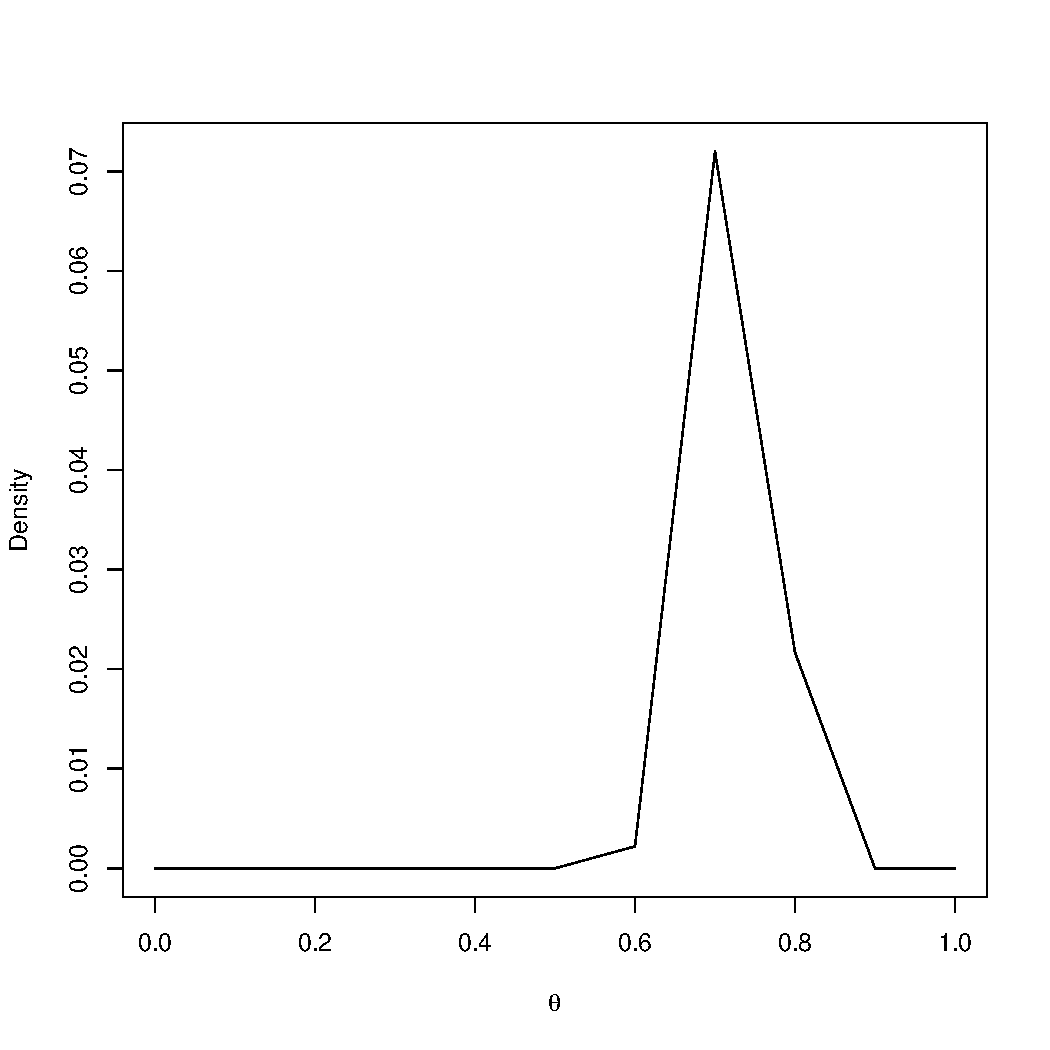
\includegraphics[width=0.7\textwidth]{binom_plot_conditional.pdf}
    \caption{Probabilities of $Y = 73$ for different values of $\theta$, $n = 100$}
    \label{fig:binom_plot_condifitional}
\end{figure}
As shown in the figure, the most probable value is $\theta = 0.7$.

\subsubsection*{Part (c)}
Under the assumption that the prior distribution $\pi(\theta)$ is uniform over its support $\mathcal{S} = \{0.0, 0.1, \ldots, 0.9, 1.0\}$ and that the likelihood function $\mathcal{L}(\theta \mid x)$ for the data is the binomial p.d.f., the posterior distribution becomes
\[
p(\theta \mid Y) 
= \frac{\mathcal{L}(Y \mid \theta) \pi(\theta)}{M(Y)}
= \frac{\mathcal{L}(Y \mid \theta) \pi(\theta)}{\sum_{\theta_i \in \mathcal S} \mathcal{L}(Y \mid \theta_i) \pi(\theta_i)}
= \frac{\binom{n}{k} \theta^k (1 - \theta)^{n - k}}{\sum_{\theta_i \in \mathcal{S}} \binom{n}{k} \theta_i^k (1 - \theta_i)^{n - k}}
= \frac{\theta^k (1 - \theta)^{n - k}}{\sum_{\theta_i \in \mathcal{S}} \theta_i^k (1 - \theta_i)^{n - k}},
\]
so that when $n = 100$, $k = 73$, we have
\[
p(\theta \mid Y) = \frac{\theta^{73} (1 - \theta)^{27}}{\sum_{\theta_i \in \mathcal{S}} \theta_i^{73} (1 - \theta_i)^{27}}.
\]
We evaluate the posterior density in \textsf{R} by
\begin{minted}{R}
    > post0 <- (theta^73 * (1 - theta)^27)/(sum(theta^73 * (1 - theta)^27))
    > print(post0)
     [1] 0.000000e+00 1.163146e-49 4.567788e-29 8.883524e-18 1.826206e-10
     [6] 1.577927e-05 2.300105e-02 7.507881e-01 2.261859e-01 9.136709e-06
    [11] 0.000000e+00
\end{minted}
and visualise it with
\begin{minted}{R}
    > plot(theta, post0, type = "l", xlab = TeX("\\theta"), ylab = "Posterior Density")
\end{minted}
\vspace*{-1cm}
\begin{figure}[H]
    \centering
    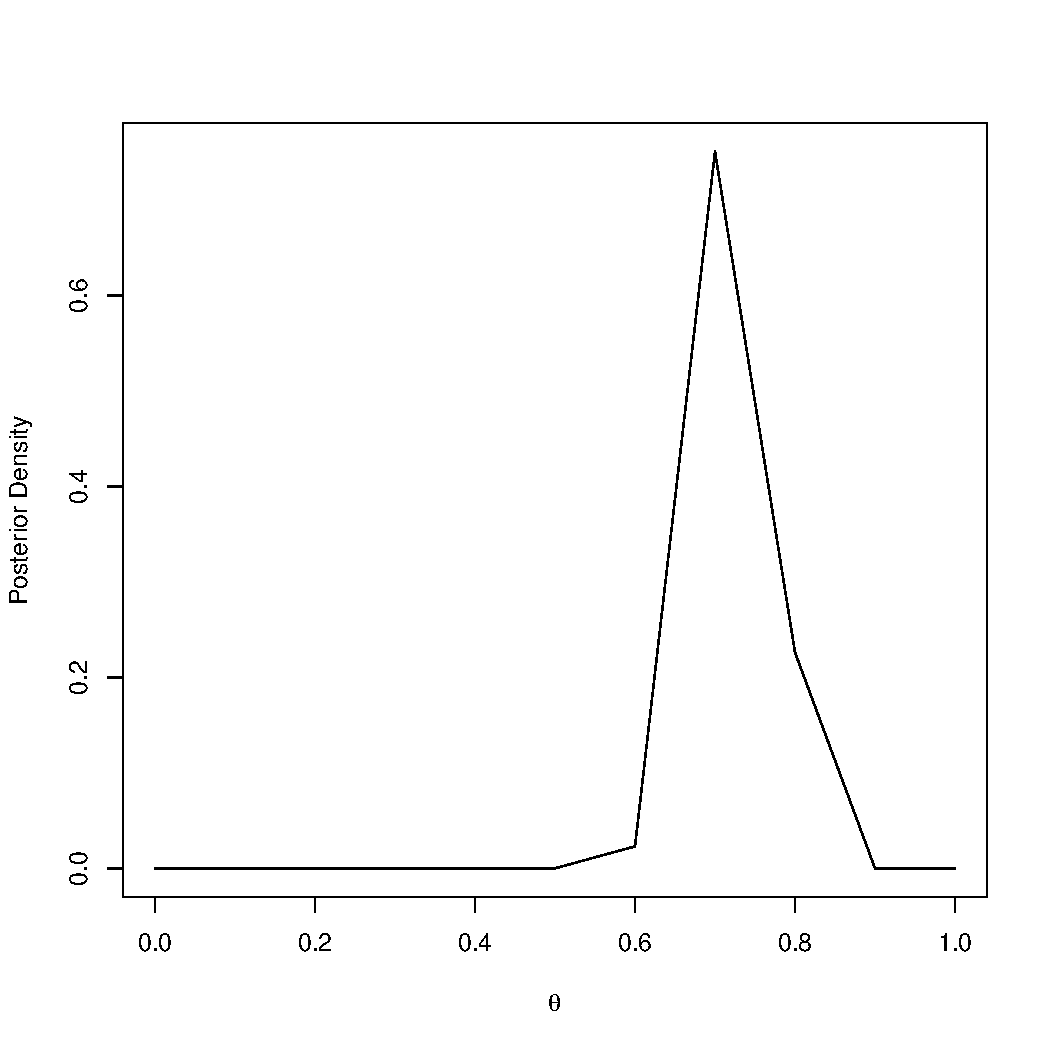
\includegraphics[width=0.7\textwidth]{binom_plot_posterior.pdf}
    \caption{Posterior density of $Y$ assuming $\pi(\theta) \sim \text{Uniform}\{0.0, 0.1, \ldots, 0.9, 1.0\}$}
    \label{fig:binom_plot_posterior_discrete}
\end{figure}

\subsubsection*{Part (d)}
Using the same likelihood function and reassigning $\pi(\theta) = 1$, we obtain the updated posterior allowing for all values of $\theta \in [0, 1]$:
\[
p(\theta \mid Y) = \frac{\theta^{73} (1 - \theta)^{27}}{\int_{\mathcal S} \theta_i^{73}(1 - \theta_i)^{27} \mathrm{d}\theta_i}
\]
We see that the marginal distribution of $Y$ resembles a beta distributed r.v. with $\alpha = 74$, $\beta = 28$. Lengthening by the coefficient of the beta distribution with the specified parameters, we obtain
\[
p(\theta \mid Y) = \frac{\frac{\Gamma(102)}{\Gamma(74)\Gamma(28)}\theta^{73}(1 - \theta)^{27}}{\int_{\mathcal S}\frac{\Gamma(102)}{\Gamma(74)\Gamma(28)} \theta_i^{73} (1 - \theta_i)^{27} \mathrm{d}\theta_i} = \frac{1}{B(74, 28)} \theta^{73} (1 - \theta)^{27}
\]
where $B(\alpha, \beta) = \frac{\Gamma(\alpha)\Gamma(\beta)}{\Gamma(\alpha + \beta)}$ is the beta function.\@ Thus we have shown that the posterior follows a beta distribution with parameters $\alpha = 74$ and $\beta = 28$. We evaluate the posterior density with \texttt{dbeta()}:
\begin{minted}{R}
    > theta <- seq(0, 1, length.out = 1000)
    > post1 <- dbeta(x = theta, shape1 = 74, shape2 = 28)
\end{minted}
and visualise them by
\begin{minted}{R}
    > plot(theta, post1, type = "l", xlab = TeX("\\theta"), ylab = "Posterior Density")
\end{minted}
\vspace*{-1cm}
\begin{figure}[H]
    \centering
    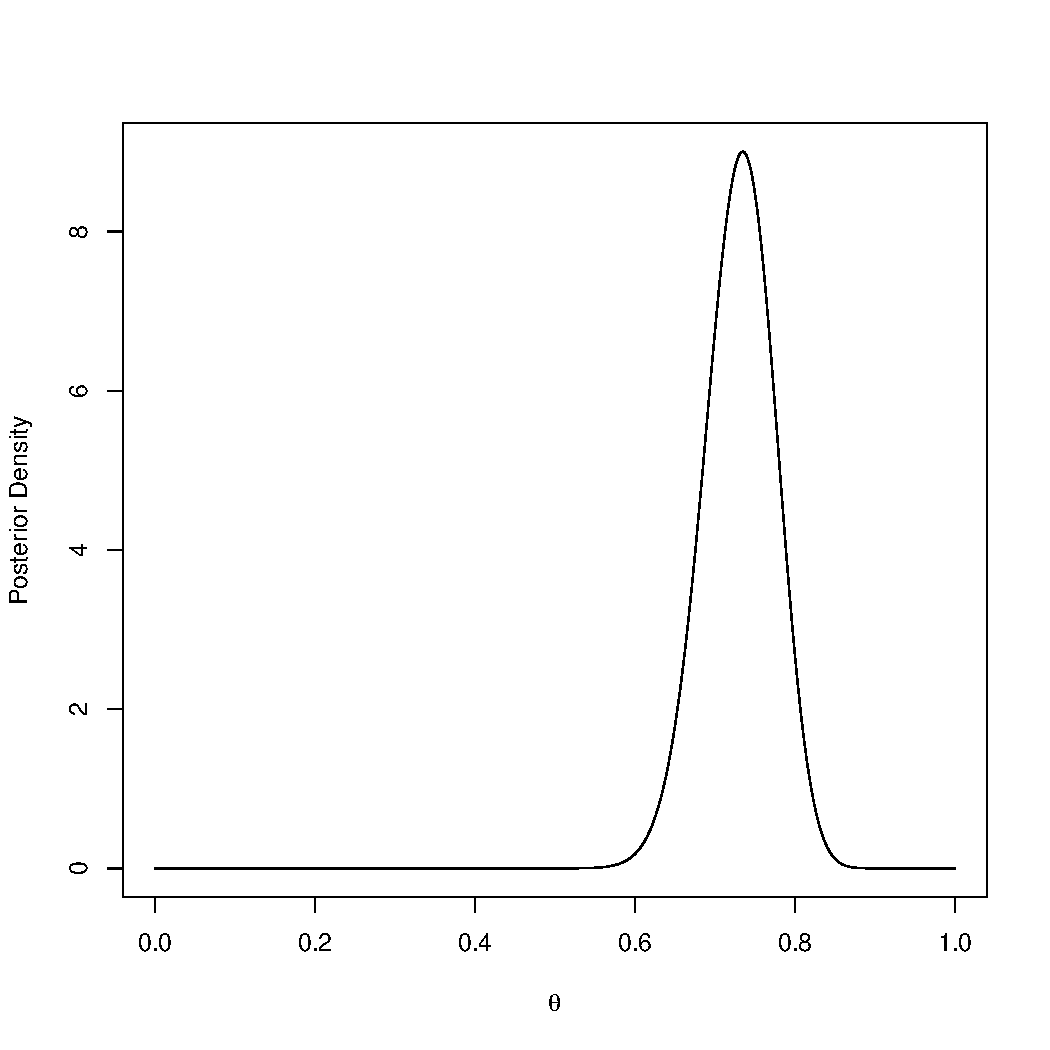
\includegraphics[width=0.7\textwidth]{binom_plot_posterior_uniform.pdf}
    \caption{Posterior density of $Y$ given the prior density $\pi(\theta) = 1$, $\theta \in [0, 1]$}
    \label{fig:binom_posterior_uniform}
\end{figure}
Figure \ref{fig:binom_posterior_uniform} displays a similar distribution to the discrete case where the centre of the distribution has shifted slightly to the right.
The maximum density is attained at $\theta = 0.7297297$ where $p(\theta \mid Y) = 9.044944$, obtained by the \textsf{R} code snippet below:
\begin{minted}{R}
    > theta[which(post1 == max(post1))]
    [1] 0.7297297
    > max(post1)
    [1] 9.044944
\end{minted}
To compute the probability $\Pr(\theta > 0.8)$, we use the \texttt{dbeta()} command in \textsf{R}:
\begin{minted}{R}
    > pbeta(q = 0.8, shape1 = 74, shape2 = 28, lower.tail = FALSE)
    [1] 0.03848785
\end{minted}
which turns out to be approximately $4\%$.

\subsubsection*{Part (e)}
Comparing Figures \ref{fig:binom_plot_posterior_discrete} and \ref{fig:binom_posterior_uniform}, we see that the distributions are similar although Figure \ref{fig:binom_plot_posterior_discrete} shows a discrete mass function whereas the distribution in Figure \ref{fig:binom_posterior_uniform} is a density. However, the most prominent difference is in the magnitude between these two distributions. This makes sense since we integrate over the distribution in (d) and summate over values of (c). As can be seen below, both turn out to equal 1:
\begin{minted}{R}
    > # (c) Sum over the probabilities
    > sum(post0)
    [1] 1
    > # (d) Evaluate the integral of 1/B(74,28) * t^74 * (1 - t)^28 dt
    > post1f <- function(t) dbeta(x = t, shape1 = 74, shape = 28)
    > integrate(post1f, lower = 0, upper = 1)$value
    [1] 1
\end{minted}
The intuitive explanation is that while we summate over the values in the discrete case (c), such that the probability mass is reflected in one-to-one proportion in the sum, we integrate in (d), which can be viewed as the limit of the infinite series
\[
\int_{\mathcal S} p(\theta \mid Y) \mathrm{d}\theta = \lim_{\ell(P_i) \to 0} \sum_{P_i \in \mathcal{P}} \ell(P_i) p(\theta = \theta_i \mid Y) \tag*{where \(\theta_i \in \overset{\circ}{P_i}\)}
\]
where $\mathcal P = \{P_i\}_{i = 1}^n$ constitutes a partition on the support $\mathcal S$, $\ell(P_i)$ yields the length of the interval $P_i$ and $\theta_i$ is an arbitrary point on the interior $\overset{\circ}{P_i}$ of $P_i$. This all goes to say that in the case (d) where we integrate over the posterior density, the densities do not enter the "sum" in one-to-one proportion, so the initial conception that the total density exceeds 1 is misfounded.\hfill\(\square\)

\newpage

\section*{Exercise 2: Random numbers, probability density functions (pdfs) and cumulative density functions (cdfs)}

The goal of this exercise is to generate random numbers, plot the histogram, the empirical pdf and cdf for these numbers, and see how they compare to the theoretical pdf and cdf. The goal is also to compare the sample mean and standard deviation to the theoretical mean and standard deviation.

\begin{enumerate}[label=(\alph*)]
    \item Generate $B = 3000$ numbers from the gamma distribution with parameters $\alpha = 2$, $\beta = 0.1$ (\textsf{R}:\texttt{rgamma}). Compute the sample mean and the sample standard deviation and compare to the theoretical mean and standard deviation (\textsf{R}:\texttt{mean,sd}).
    \item Plot the theoretical density (pdf) of the gamma distribution (\textsf{R}:\texttt{dgamma}). Plot empirical density based on the data on the same graph. In \textsf{R} one can use
    \begin{minted}{R}
    library(lattice)
    densityplot(y)
    \end{minted}
    given that \texttt{y} are the data. Plot the histogram on another graph (\textsf{R}:\texttt{histogram}).
    \item Plot the theoretical cumulative density function (cdf) of the gamma distribution (\textsf{R}:\texttt{pgamma}). Plot empirical cumulative density based on the data on the same graph. In \textsf{R} one can use
    \begin{minted}{R}
    n <- length(y)
    y_sort <- sort(y)
    plot(y_sort, (1:n)/n, type = "s", ylim = c(0,1))
    \end{minted}
    where again \texttt{y} are the data.
\end{enumerate}

\subsection*{Solution}

\subsubsection*{Part (a)}
Start with the random number generation, with the RNG seed set to 42 for reproducibility:
\begin{minted}{R}
    > y <- rgamma(n = 3000, shape = 2, rate = 0.1)
\end{minted}
Compare theoretical and sample moments:
\begin{minted}{R}
    > # Theoretical mean
    > 2 / 0.1
    [1] 20
    > # Sample mean
    > mean(y)
    [1] 19.87275
    > # Theoretical variance
    > 2 / 0.1^2
    [1] 200
    > # Sample variance
    > var(y)
    [1] 202.2949
\end{minted}
We see that the theoretical and sample moments are very similar, with a difference of $0.12725$
between the theoretical and sample mean, and a difference of $2.29486$ between the theoretical and sample mean. In fact, as $n$ increases, we would expect these estimates to become even better by the law of large numbers.

\subsubsection*{Part (b)}
The following code snippet was used to generate the plot below in Figure \ref{fig:plot_theoretical_empirical}:
\begin{minted}{R}
    > t <- seq(min(y), max(y), length.out = 3000)
    > ft <- dgamma(x = t, shape = 2, rate = 0.1)
    > 
    > par(mfrow = c(1, 2))
    > plot(density(y), main = NA, xlab = "Y", col = "blue", ylim = range(ft, density(y)$y))
    > lines(t, ft, col = "red")
    > legend("topright", inset = c(0.05, 0.05), legend = c("Theoretical", "Sample"), 
    + col = c("blue", "red"), lty = 1)
    > hist(y, main = NA, xlab = "Y")
\end{minted}

\begin{figure}[H]
    \centering
    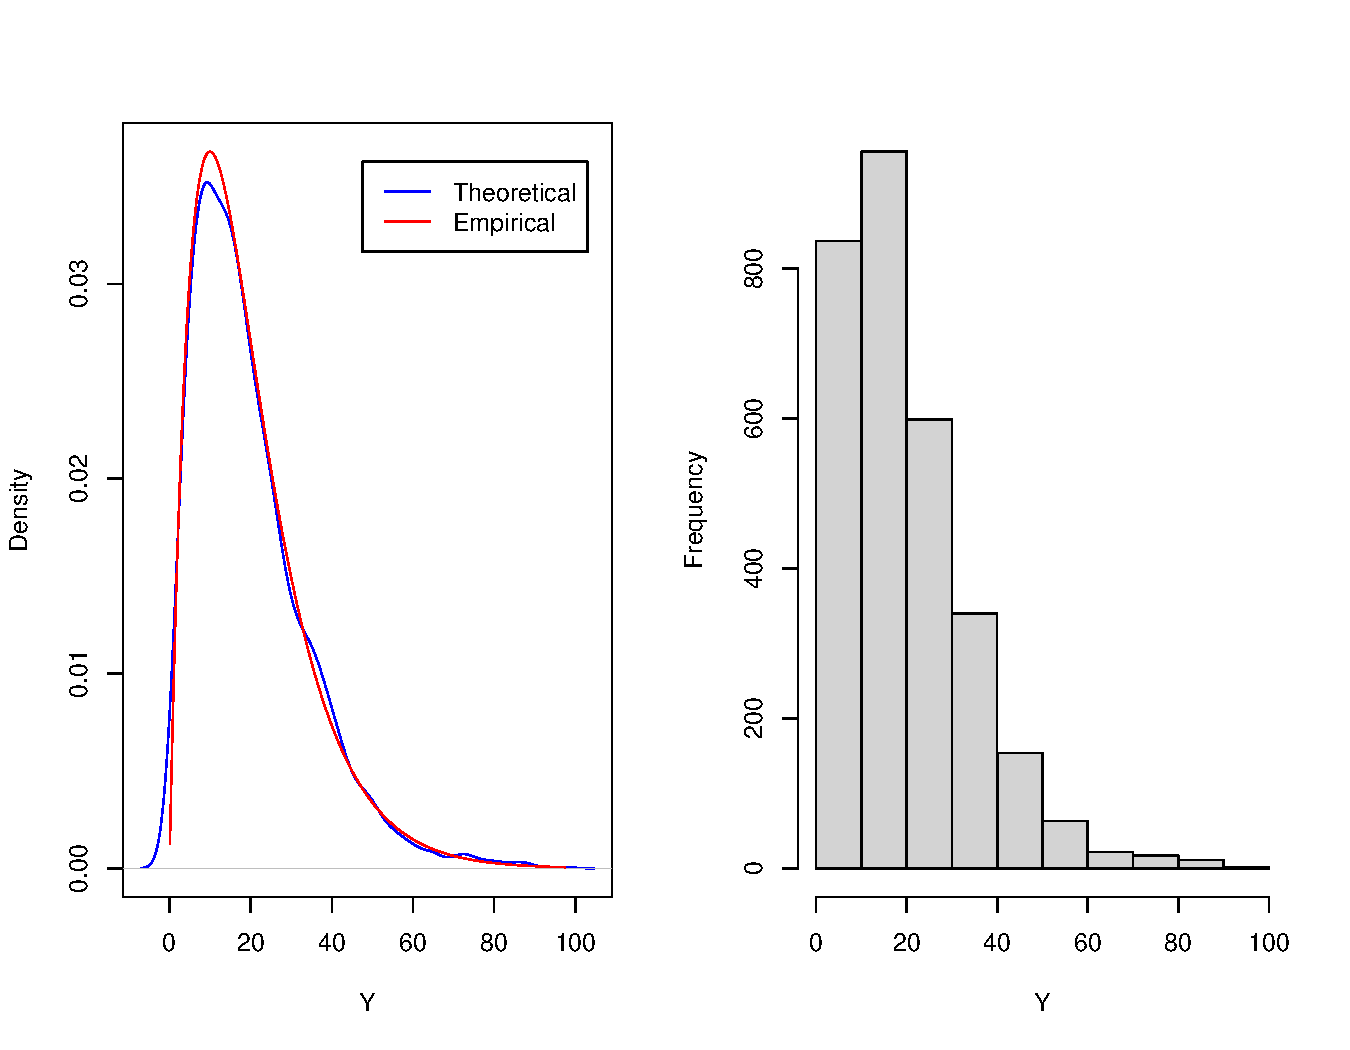
\includegraphics[width=\textwidth]{plot_theoretical_empirical.pdf}
    \caption{Comparisonal plot of the theoretical and empirical densities}
    \label{fig:plot_theoretical_empirical}
\end{figure}

\subsubsection*{Part (c)}
The code below was used to create the plot shown in Figure \ref{fig:comparison_ecdf_tcdf}:
\begin{minted}{R}
    > n <- length(y)
    > ecdf <- sort(y)
    > tcdf <- pgamma(q = t, shape = 2, rate = 0.1)
    >
    > plot(ecdf, 1:n/n, type = "s", ylim = c(0, 1), col = "blue", xlab = "Y", 
    + ylab = "Cumulative Density")
    > lines(t, tcdf, col = "red")
    > legend("topright", inset = c(0.05, 0.05), legend c("Theoretical", "Empirical"), 
    + col = c("blue", "red"), lty = 1)
\end{minted}
\begin{figure}[H]
    \centering
    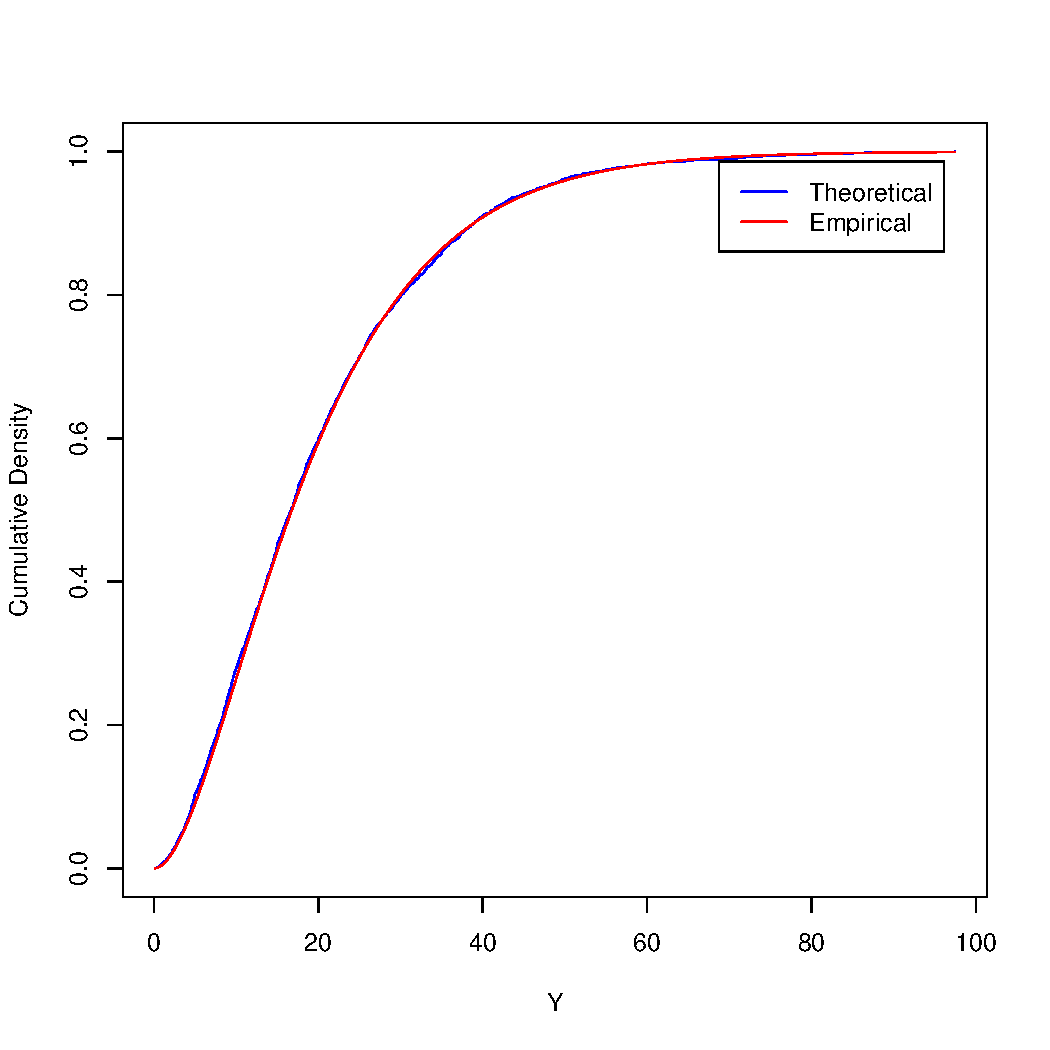
\includegraphics[width=0.7\textwidth]{comparison_ecdf_tcdf.pdf}
    \caption{Comparison of the theoretical and empirical cumulative density functions.}
    \label{fig:comparison_ecdf_tcdf}
\end{figure}

We see that in both (b) and (c), the distributions match closely, which is consistent since the sample vector $\mathbf{y} = \{y_1, \ldots, y_{3000}\}$ was drawn from the theoretical distribution and should therefore resemble it with increasing precision as $B$ grows larger.
\end{document}